\section{Further information for baryonic Zprime Model}

\subsection{Cross-section scaling}

The dependence of the cross section of the $pp \rightarrow H\chiDM\bar{\chiDM}+X$ process 
on $g_{h \Zprime \Zprime}$ is shown in Figure~\ref{fig:vectorXSdeps}. 
The curves have been fit to second-order polynomials, where $y$ is the cross-section
and $x$ is the coupling $g_{h \Zprime \Zprime}$. 

For $m_{med} = 100$~\gev, the fit function is 
$$y = -0.12 - 3.4\times10^{-3}x + 2.7\times10^{-4}x^2$$.
For $m_{med} = 1$~\tev, the fit function is 
is $$y = 0.0012 - 2.4\times10^{-7}x + 1.5\times10^{-7}x^2$$,

\be
y = -0.12 - 3.4\times10^{-3}x + 2.7\times10^{-4}x^2.
\ee
For $\mMed = 1$ TeV, the fit function is 
is:

\be
y = 0.0012 - 2.4\times10^{-7}x + 1.5\times10^{-7}x^2.
\ee

\begin{figure}[hbpt!]
	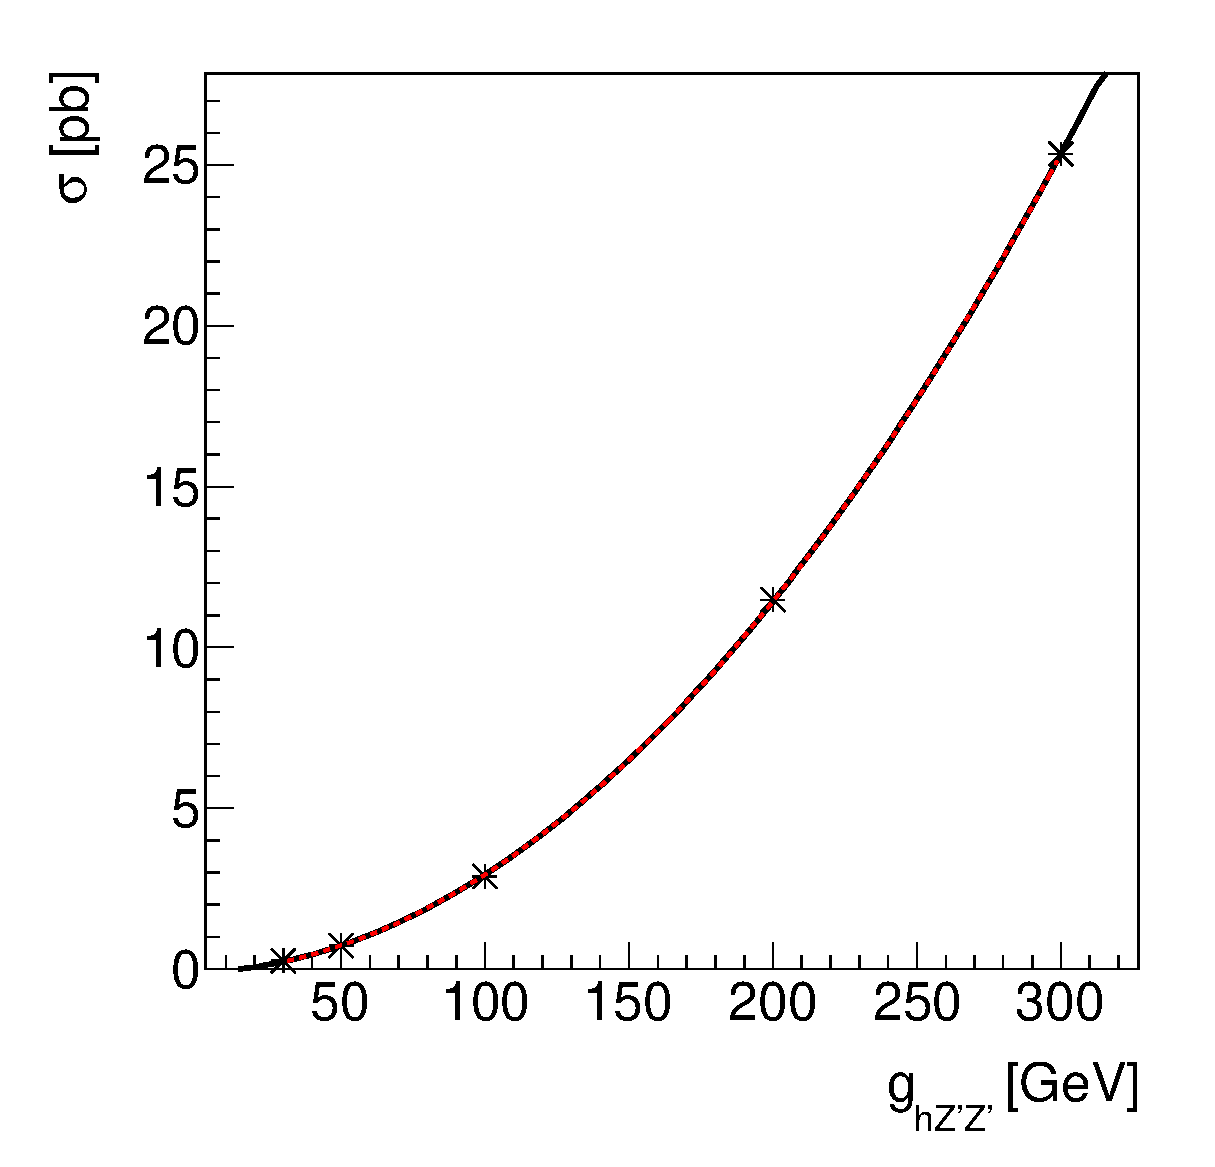
\includegraphics[width=0.99\linewidth]{figures/EW/monoH/zprime_xs_med_100}\\
	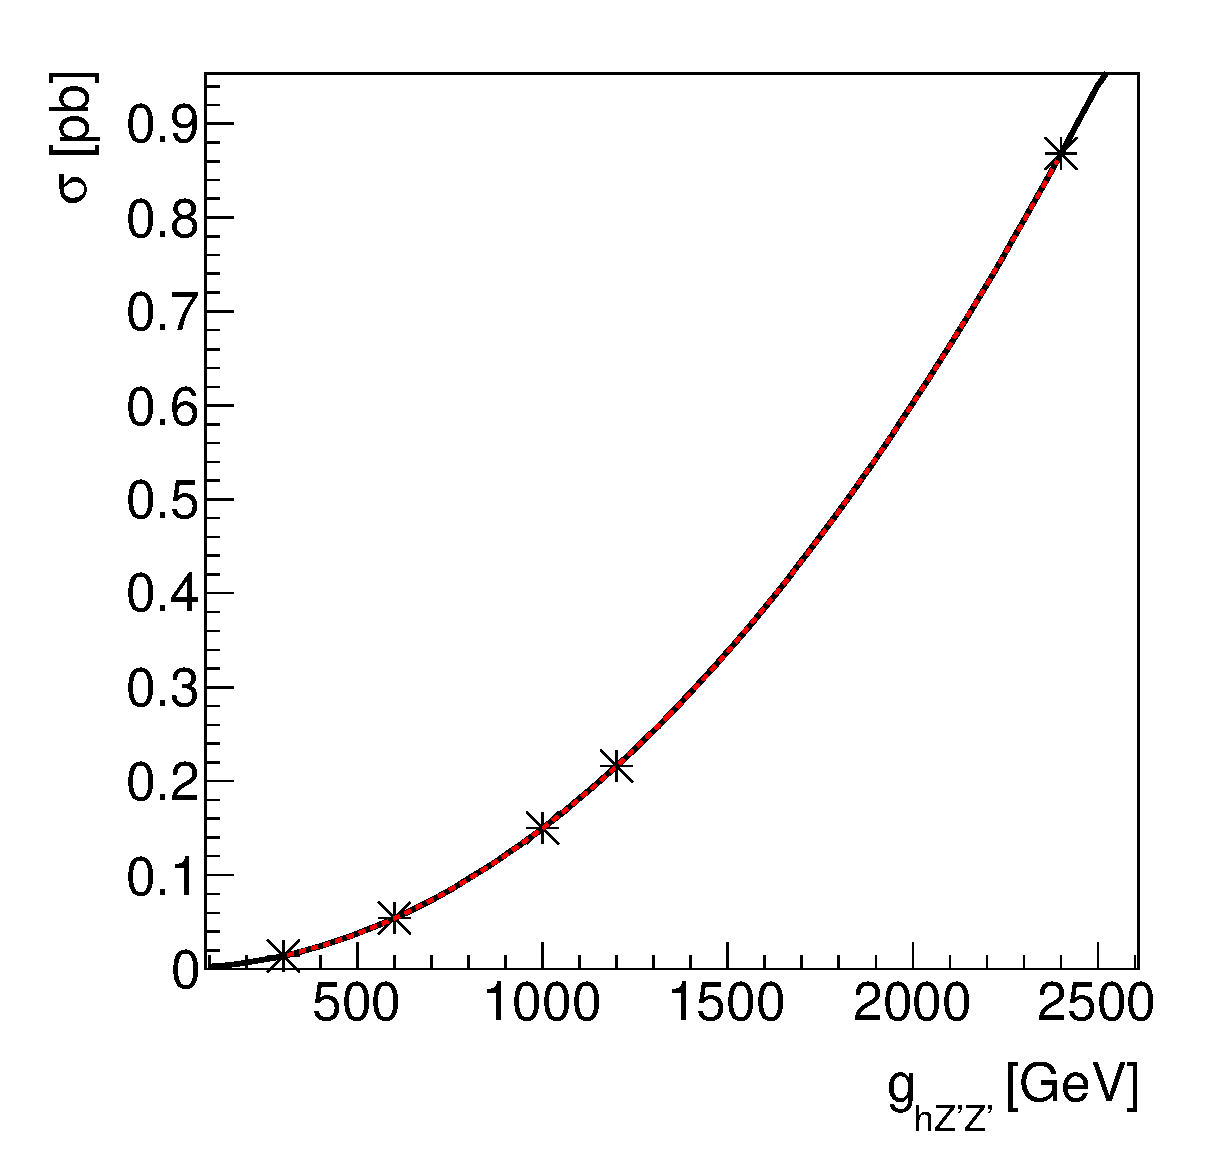
\includegraphics[width=0.99\linewidth]{figures/EW/monoH/zprime_xs_med_1000}
	\caption{Cross section of the $pp \rightarrow H\chiDM\bar{\chiDM}$ process as a function of 
		$g_{h \Zprime \Zprime}$ for $m_{\Zprime} = 100$~\gev (left) 
		and $m_{\Zprime} = 1$~\tev (right). The fit functions are shown in the text. 
		\label{fig:vectorXSdeps}}
\end{figure}

